\section{Diseño e implementación}

El diseño del trabajo práctico se separó en partes distinguidas: primero conseguir una gramática básica razonable y luego implementar los procesos propuestos por la materia. Para esto el uso de PLY como parser generator simplificó gratamente el proceso.

\subsection{Lexer}

Si bien el lexer y el parser se desarrollaron en conjunto el enfoque fué en tener a éste terminado primero. Dado que un conjunto de tokens suficientemente expresivo y estable nos permitió iterar con las reglas del parser mucho más fácilmente.

Los tokens nuestro lexer genera son los siguientes:
\begin{itemize}
    \item BEGIN\_DESCRIPTOR: El inicio de un descriptor, siempre es la cadena ``[''
    \item DESCRIPTOR\_VALUE: Una cadena de texto arbitrario (excepto el caracter para comillas dobles) entre comillas dobles
    \item END\_DESCRIPTOR: El fin de un descriptor, siempre es la cadena ``]''
    \item BEGIN\_COMMENT: El inicio de un comentario, siempre es la cadena ``{''
    \item END\_COMMENT: El fin de un comentario, siempre es la cadena ``}''
    \item MOVE\_NUMBER: Un número válido para un movimiento, cómo ``1...'' o ``2.''
    \item MOVE: Un movimiento válido
    \item GAME\_RESULT: El resultado de una partida
    \item WORD : Cualquier otra cadena sin espacios en el medio
\end{itemize}
    
    
Una cosa a notar es que nuestro lexer aprovecha el que el motor de expresiones regulares permite priorizar opciones ordenándolas (por ejemplo \verb/a|aa/ nunca matchea aa). Utilizamos esto para tener una buena definición de WORD. Otra cosa notable es que podríamos haber armado a los descriptores como un único token (algo parecido a \verb/\[([^" \t]+)[ \t]*"([^"]*)"\]/ )  pero dado que decidimos ``congelar'' el desarrollo del lexer ni bien sentíamos que alcanzaba para nuestras necesidades nos quedamos con un poco de complejidad extra.

La existencia del token WORD es para poder tokenizar el texto arbitrario dentro de comentarios. Una alternativa es la de "island grammars" propuesta por ANTLR o el uso de start conditions presentes en PLY.

\subsection{Parser}


El el desarrollo del parser fué principalmente top-down. Comenzando por la regla pgn\_file fuimos describiendo la forma del archivo (un archivo pgn es una lista de partidas, que son un encabezado y un cuerpo, un encabezado es una lista de descriptores...). Dos cosas a puntualizar son el que tenemos muchas reglas con la forma lista\_de\_cosas -> cosa lista\_de\_cosas | cosa y que para el manejo de algunos errores construimos reglas que producen la terminación del programa al reducir.

La lista de reglas definidas es la siguiente:

  \begin{itemize}
    \item pgn\_file: Un fichero pgn el símbolo inicial de nuestra gramática
    \item pgn\_game\_list: Una lista de partidos
    \item pgn\_game: Un partido, compuesto por si header y la descripción propia del partido
    \item descriptor\_list: El encabezado del archivo, una lista de descriptores
    \item descriptor: Una etiqueta específica de un archivo
    \item any\_token: El nombre de una etiqueta. Está conformado de todos los tokens posibles dado que quisimos permitir movimientos o cadenas como nombres válidos
    \item game: Las jugadas que conforman a un partido seguidas de su resultado
    \item turn\_list: Una lista de jugadas
    \item move: Una jugada en específico, posee al menos un movimiento de pieza
    \item move\_content: Una secuencia de comentarios y movimientos de piezas que corresponden a una jugada
    \item comment: Un comentario
    \item comment\_words\_list: La lista de palabras, jugadas y subcomentarios que conforman a un comentario
    \item comment\_word: Un elemento de un comentario (un comentario o una palabra)
    \item any\_comment\_token: Una palabra de un comentario
\end{itemize}  
    
    
    

\begin{sidewaysfigure}[ht]
    \centering
    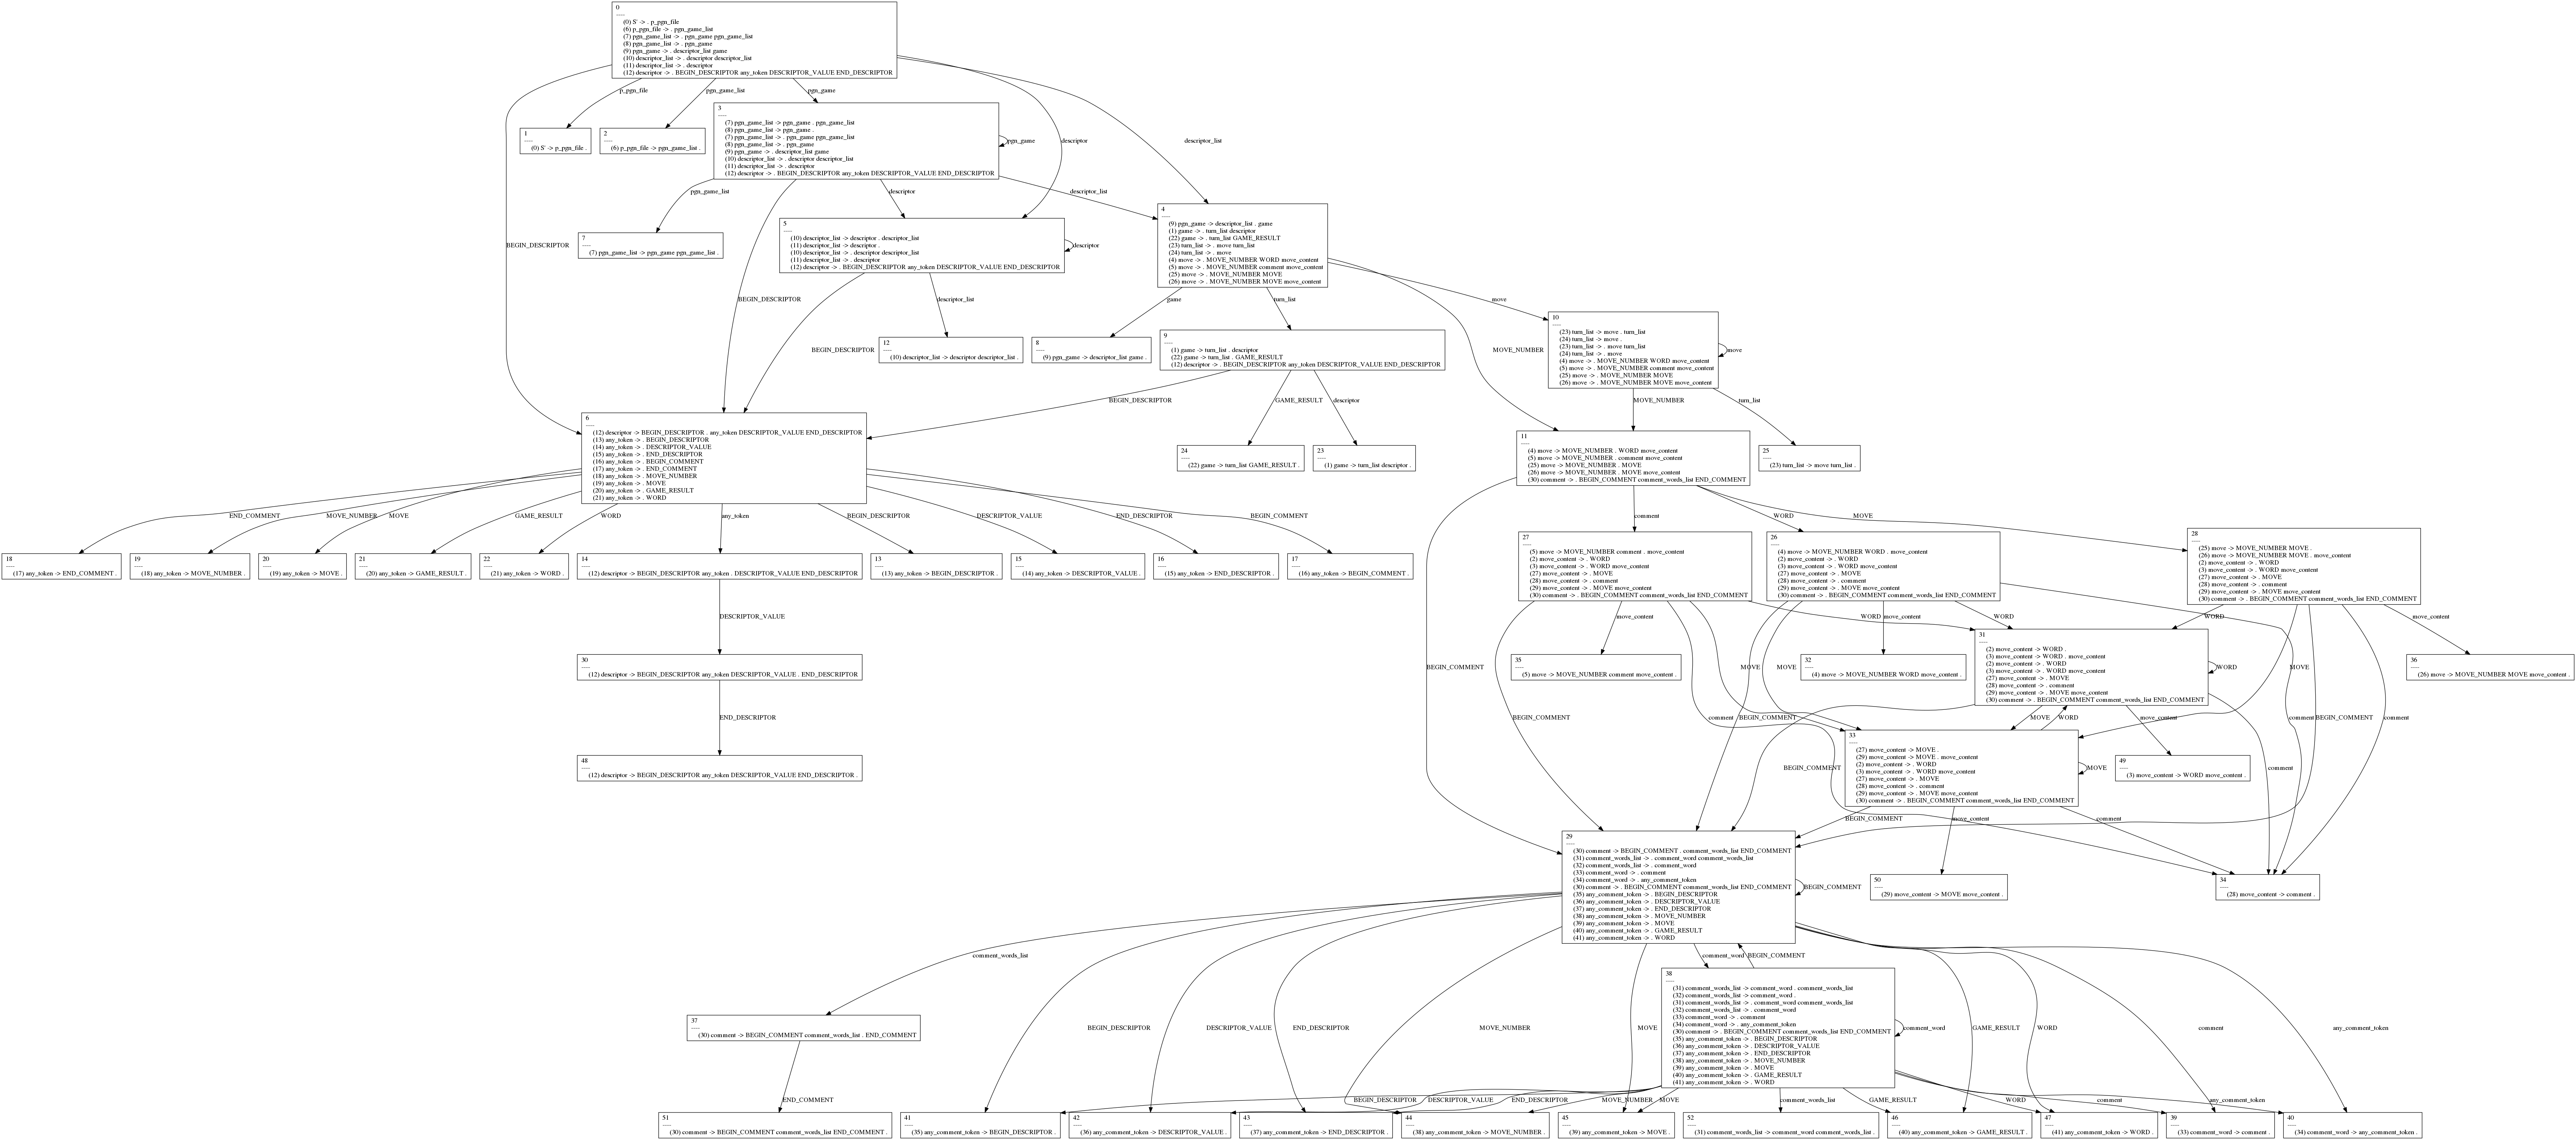
\includegraphics[scale=0.09]{images/automata.png}
    \caption{Autómata de gramática.}
\end{sidewaysfigure}